\documentclass[letterpaper, 10 pt, conference]{ieeeconf}
% IEEE Robotics and Automation Letters, initial submission. RAS template ieeeconf.cls
% (https://ras.papercept.net/conferences/support/files/ieeeconf.zip); the final version moves to
% \documentclass[letterpaper, 10 pt, journal, twoside]{IEEEtran}. Limit: 6 pages including figures and
% references, up to 2 more at a charge. Review is double-anonymous: no author names, affiliations,
% acknowledgment, vehicle name or lab logos until acceptance.
\IEEEoverridecommandlockouts
\overrideIEEEmargins

\usepackage[T1]{fontenc}
\usepackage[utf8]{inputenc}
\usepackage{cite}
\usepackage{graphicx,color}
\usepackage{textcomp}
\usepackage{amsmath}
\usepackage{amsfonts}
\usepackage{amssymb}
\usepackage{booktabs}
\usepackage{multirow}
\usepackage{makecell}
\usepackage{nicefrac}
\usepackage{xcolor}
\usepackage{xspace}
\usepackage{microtype}
\usepackage{url}
\usepackage[hidelinks]{hyperref}
\usepackage[scaled=0.92]{helvet} % sans font for figures/architecture.tex
\usepackage{tikz}
\usetikzlibrary{arrows.meta,calc,positioning,fit}
\makeatletter\def\@IEEEsectpunct{\ \,}\makeatother % no class colon after run-in headings, whose titles end in a period

% Custom macros
\newcommand{\method}{EgoPed\xspace}
\newcommand{\fullseq}{Full-seq\xspace}
\xspaceaddexceptions{+} % \method+IA, not \method +IA
\newcommand{\eg}{e.g.,\xspace}
\newcommand{\ie}{i.e.,\xspace}
\newcommand{\etal}{\textit{et al.}\xspace}
\newcommand{\TODO}[1]{{\textcolor{red}{{#1}}}} % TODOs in red
\newcommand{\ci}[2]{\,{\scriptsize[#1,\,#2]}}

\newif\ifanonymous
\anonymoustrue % double-anonymous review; \anonymousfalse restores authors and acknowledgment

\title{\LARGE \bf EgoPed: Ego-Conditioned Pedestrian Body Motion Generation via Latent Diffusion}

\ifanonymous
\author{Anonymous Authors}
\else
\author{Erik Sch\"utz, Mohan Ramesh and Fabian B. Flohr%
\thanks{The authors are with the Intelligent Vehicles Lab, Munich University of Applied Sciences, Munich, Germany
  {\tt\small erik.schuetz@hm.edu}}}
\fi

\makeatletter % \bstctlcite from IEEEtran.cls 1.8
\def\bstctlcite{\@ifnextchar[{\@bstctlcite}{\@bstctlcite[@auxout]}}
\def\@bstctlcite[#1]#2{\@bsphack\@for\@citeb:=#2\do{\edef\@citeb{\expandafter\@firstofone\@citeb}\if@filesw\immediate\write\csname #1\endcsname{\string\citation{\@citeb}}\fi}\@esphack}
\makeatother

\begin{document}
\bstctlcite{IEEEexample:BSTcontrol}

% Teaser on the first page, below the title block: figure* cannot float onto page 1.
\makeatletter
\let\egoped@maketitle\@maketitle
\def\@maketitle{\egoped@maketitle
  \begin{minipage}{\textwidth}
  \def\@captype{figure}
  \setcounter{figure}{0}% ieeeconf typesets the title block twice
  \centering
  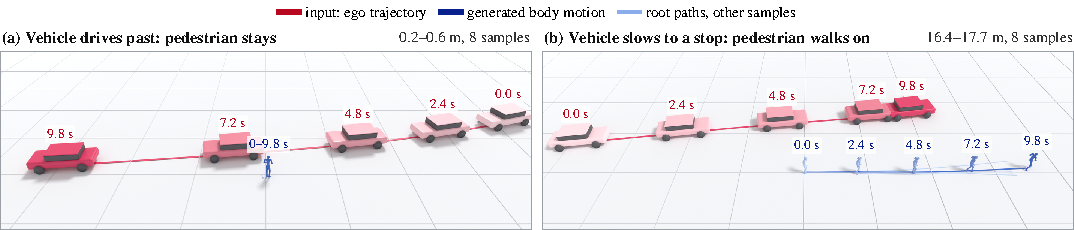
\includegraphics[width=\textwidth]{figures/teaser.pdf}
  \caption{\method generates full-body pedestrian motion from the ego vehicle's trajectory alone, given in the pedestrian's initial frame. Panels (a) and (b) share model and noise and differ only in the input trajectory. Titles give the distance travelled across 8 noise seeds, time stamps pair vehicle and pedestrian, and the grid spacing is 5\,m. Both validation conditions were chosen for illustration. Section~\ref{sec:main} measures the coupling over the whole test set.}
  \label{fig:teaser}
  \end{minipage}\vspace{2mm}}
\makeatother

\maketitle
\thispagestyle{empty}
\pagestyle{empty}

\begin{abstract}
Simulation-based testing of automated vehicles needs pedestrians whose whole-body motion depends on the vehicle, yet existing motion generators condition on text, waypoints, goals or the static scene. We present \method, a latent diffusion model that generates 3D full-body pedestrian motion directly from the ego vehicle's trajectory, encoded by a pretrained, frozen trajectory encoder into a single token. On 5{,}668 paired sequences from nuScenes, Waymo and our staged recordings, mirrored and split by scene, \method lowers the root displacement error of a trained unconditional prior from 3.11 to 2.43\,m and lifts the coupling between generated and recorded stopping decisions (Ego-Coupling Score) from 0.02 to 0.31. The Fréchet distance is blind to this coupling. An ego-blind prior matches the best conditional model, and the two design choices it favours both raise mean trajectory error. We therefore propose per-condition trajectory error and the Ego-Coupling Score, with scene-clustered statistics across seeds, to evaluate this task. The coupling is observational. It rests mostly on pedestrians who stand and partly on scene geometry, and the body labels are a lightly articulated template.
\end{abstract}

% RA-L wants the keywords beneath the abstract; the first two come from the RA-L list.
% ieeeconf locks out the keywords environment in conference mode, so they are set by hand.
{\small\bfseries\noindent\textit{Index Terms}---Human and Humanoid Motion Analysis and Synthesis, Intelligent Transportation Systems, Deep Learning Methods, Modeling and Simulating Humans, Performance Evaluation and Benchmarking.\par}


%----------------------------------------------------------------------
\section{INTRODUCTION}
%----------------------------------------------------------------------

Generating realistic pedestrian body motion is a core capability for automated-vehicle (AV) simulation.
Simulation pipelines need diverse, plausible pedestrian behaviour to stress-test perception and planning, especially in the long tail of close-range encounters that are unsafe or impractical to collect on the road.
That behaviour is coupled to the vehicle, whose speed, path and proximity influence whether a pedestrian crosses, waits, accelerates or turns~\cite{camara2021pedmodels2}, and benchmarks such as JAAD~\cite{rasouli2017jaad} and PIE~\cite{rasouli2019pie} annotate exactly that dependence.
The models built on them, however, predict a discrete event or a ground-plane path~\cite{alahi2016sociallstm,salzmann2020trajectron,gu2022mid}, not an articulated body.
The same gap exists for mobile robots that share pavements with people, whose simulators also need pedestrians that react to the robot.

Full-body human motion synthesis has meanwhile advanced quickly through text-conditioned diffusion~\cite{chen2023mld,tevet2023mdm,zhang2022motiondiffuse,guo2024momask}.
These generators are blind to the vehicle in the way a simulator cannot afford. A person crossing a street is generated the same whether a car approaches at 50\,km/h or stands still.
Pedestrian-specific generators control the body through waypoints, goals or the static scene~\cite{rempe2023tracepace,liu2025pedgen}, and concurrent work reaches the body only through an intermediate 2D path and a text prompt~\cite{liu2026controlped}.

We present \method, which generates the body motion directly from the ego vehicle's trajectory (Fig.~\ref{fig:teaser}).
It builds on Motion Latent Diffusion (MLD)~\cite{chen2023mld} and replaces the text condition with a pretrained, frozen trajectory encoder whose output is pooled into a single conditioning token.
Most of this paper is about showing that such a model \emph{uses} the vehicle.
The condition belongs to another agent and never determines the output, so the standard Fréchet distance (FID), which compares the marginal distribution of generated and real motion, can be excellent for a model that ignores the vehicle altogether.
We therefore evaluate every model on per-condition root trajectory error and on an Ego-Coupling Score that measures whether generated stopping decisions follow the vehicle, with three training seeds for each main model, a test split that shares no scene with training, and a significance rule fixed before the test split was touched.

We make three contributions.
\begin{enumerate}
\item \textbf{Ego-conditioned body motion.} To our knowledge the first model that generates 3D pedestrian body motion directly from the ego-vehicle trajectory. Against a separately trained unconditional prior it lowers root trajectory error by 0.68\,m and raises the Ego-Coupling Score from 0.02 to 0.31.
\item \textbf{Conditioning-aware evaluation.} Per-condition trajectory error and the Ego-Coupling Score, with scene-clustered statistics across seeds. With them we show that FID cannot see the conditioning. An ego-blind prior matches the best conditional FID, and both design choices FID prefers raise the mean trajectory error.
\item \textbf{Data and its limits.} 5{,}668 paired ego--pedestrian sequences, 11{,}336 with their mirrored copies, from nuScenes~\cite{caesar2020nuscenes}, Waymo~\cite{sun2020waymo} and staged recordings of our research vehicle, split by scene, and a reference-free audit showing that the body poses are a canonical template sliding along the root path.
\end{enumerate}

%----------------------------------------------------------------------
\section{RELATED WORK}
\label{sec:related}
%----------------------------------------------------------------------

\subsection{Pedestrian Behaviour and Trajectory Prediction}

Video benchmarks predict discrete events such as crossing~\cite{rasouli2017jaad,rasouli2019pie}, and reported gains depend strongly on evaluation design~\cite{kotseruba2021benchmark}. Trajectory predictors treat pedestrians as points on the ground plane~\cite{rudenko2020survey}, from social pooling~\cite{alahi2016sociallstm} to attention over heterogeneous agents~\cite{salzmann2020trajectron} and diffusion~\cite{gu2022mid}. Trajectron++~\cite{salzmann2020trajectron} can also condition the forecast on the ego vehicle's planned future. We keep this literature's displacement metrics for the root of the body and add an articulated body on top.

\subsection{Human Motion Synthesis and Control}

HumanML3D and its 263-dimensional motion representation~\cite{guo2022humanml3d}, which we adopt, made language the standard condition for 3D motion generation. Diffusion~\cite{ho2020ddpm,song2021ddim} with classifier-free guidance~\cite{ho2022cfg} now dominates. MDM~\cite{tevet2023mdm} and MotionDiffuse~\cite{zhang2022motiondiffuse} denoise raw motion, MLD~\cite{chen2023mld} denoises in the latent space of a motion VAE, following latent diffusion for images~\cite{rombach2022sd}, and token-based generators~\cite{guo2024momask} are an alternative. Spatial control~\cite{karunratanakul2023gmd,xie2024omnicontrol} constrains where the generated person's own body should be, while models conditioned on the scene~\cite{hassan2021samp,jiang2024trumans} or a partner~\cite{liang2024intergen} respond to static geometry or a second human. Our condition differs in kind. It is the trajectory of a different, independently moving agent that only shapes a distribution over plausible reactions. Frozen conditioning encoders are standard in image generation~\cite{rombach2022sd}, and we test whether freezing matters here.

\subsection{Pedestrian Motion Generation for Driving Scenes}

Trace and Pace~\cite{rempe2023tracepace} combines a trajectory diffusion model, guided by waypoints, speed and social groups, with a physics-based humanoid controller. PedGen~\cite{liu2025pedgen} learns full-body pedestrian motion from noisily labelled web videos, with scene, goal and body shape as context. Neither is controlled by the trajectory of a vehicle. Concurrent work, ControlPed~\cite{liu2026controlped}, conditions a 2D pedestrian trajectory on surrounding vehicles and lifts it to body motion with a text-conditioned diffusion model, so the body sees the vehicle only through that trajectory and the prompt. Section~\ref{sec:pedgen} compares \method with PedGen.

\subsection{Evaluating Conditional Generative Models}

Fréchet distances compare generated and real samples through the statistics of a pretrained feature extractor~\cite{heusel2017fid}, for motion a motion encoder~\cite{guo2022humanml3d}. Their known failure modes concern how faithfully they measure the \emph{marginal}, such as estimator bias~\cite{chong2020unbiasedfid}, preprocessing~\cite{parmar2022cleanfid} and the extractor's own class structure~\cite{kynkaanniemi2023imagenetfid}. The problem we document is orthogonal. A score can measure the marginal well and say nothing about whether the condition was used. Estimated body motion is also known to be physically imperfect~\cite{rempe2020contact,yuan2023physdiff}, and we measure how imperfect our labels are.

%----------------------------------------------------------------------
\section{METHOD}
\label{sec:method}
%----------------------------------------------------------------------

\begin{figure*}[t]
  \centering
  \resizebox{\linewidth}{!}{% EgoPed architecture figure (TikZ). Grounded in:
%   mld/models/architectures/ego_encoder.py   (EgoEncoder: Linear 2->256, sin. PE, 4x TransformerEncoderLayer, 4 heads, LayerNorm)
%   pretrain_ego_encoder.py                   (mean-pooled, projected ego tokens vs. mean-pooled VAE posterior mean; MSE + 0.1 (1 - cos))
%   EgoEncoderPooled                          (masked mean-pool + 2-layer projection head -> one 256-D token)
%   mld/models/architectures/mld_denoiser.py  (arch=trans_enc via configs/modules/denoiser.yaml: [z_t | t_emb | c_bar] -> learned PE
%                                              -> 9-layer SkipTransformerEncoder, 4 heads -> first L=4 tokens)
%   mld/models/modeltype/mld.py               (frozen ego encoder; CFG by zeroing the ego input w.p. 0.1; frozen VAE decode)
% Requires: \usepackage{tikz} \usetikzlibrary{arrows.meta,calc,positioning,fit}
\definecolor{ink}{HTML}{1F2A37}
\definecolor{egofill}{HTML}{FAD9A9}\definecolor{egoedge}{HTML}{D48A2A}\definecolor{egotok}{HTML}{EFA54A}
\definecolor{denfill}{HTML}{D4E4F4}\definecolor{denedge}{HTML}{4F82BE}\definecolor{lattok}{HTML}{6E9BD0}
\definecolor{vaefill}{HTML}{EFEFEF}\definecolor{vaeedge}{HTML}{8A8A8A}\definecolor{timetok}{HTML}{BDBDBD}
\definecolor{motfill}{HTML}{CFE6D3}
\begin{tikzpicture}[
  font=\sffamily\scriptsize,
  >={Stealth[length=4pt,width=3.5pt]},
  line/.style={->,draw=ink,line width=0.6pt},
  stage/.style={draw,rounded corners=3pt,line width=0.7pt,align=center,inner sep=3pt,minimum height=11mm},
  enc/.style={stage,fill=egofill,draw=egoedge},
  den/.style={stage,fill=denfill,draw=denedge},
  vae/.style={stage,fill=vaefill,draw=vaeedge,dashed},
  op/.style={draw=ink!70,rounded corners=2pt,line width=0.5pt,fill=white,align=center,inner sep=2.5pt},
  lbl/.style={align=center,inner sep=1pt,text=ink},
  num/.style={circle,draw=ink,fill=white,line width=0.5pt,inner sep=0.6pt,font=\sffamily\tiny\bfseries},
  panel/.style={font=\sffamily\footnotesize\bfseries,anchor=west,inner sep=0pt},
]

% ---------- helpers ----------
% \tokrow{x}{y}{n}{fill}{name}: n adjacent token squares, left edge at x, centred on y
\newcommand{\tokrow}[5]{%
  \foreach \k in {1,...,#3}{%
    \draw[fill=#4,draw=ink,line width=0.35pt] ($(#1,#2)+({(\k-1)*0.2},-0.1)$) rectangle ++(0.2,0.2);}%
  \node[inner sep=0pt,fit={(#1,#2-0.1) ($(#1,#2)+({#3*0.2},0.1)$)}] (#5) {};}
% \grid{x}{y}{cols}{rows}{fill}{name}: small input grid (time along x)
\newcommand{\grid}[6]{%
  \foreach \i in {1,...,#3}{\foreach \j in {1,...,#4}{%
    \draw[fill=#5,draw=ink,line width=0.3pt] ($(#1,#2)+({(\i-1)*0.16},{-(\j-1)*0.16})$) rectangle ++(0.16,-0.16);}}%
  \node[inner sep=0pt,fit={(#1,#2) ($(#1,#2)+({#3*0.16},{-#4*0.16})$)}] (#6) {};}

% =====================================================================
% (a) Ego-encoder pretraining
% =====================================================================
\node[panel] at (0,0.35) {(a) Ego-encoder pretraining};

% row 1: ego trajectory -> ego encoder -> c -> mean-pool
\grid{0.15}{-0.55}{8}{2}{white}{egoA}
\draw[->,ink!70,line width=0.4pt] ($(egoA.north west)+(0,0.12)$) -- ($(egoA.north east)+(0,0.12)$) node[midway,above=-1pt,font=\sffamily\tiny,text=ink!80] {time};
\node[lbl,below=1pt of egoA] {ego trajectory $\mathbf{e}$\\$196\times2$};
\node[enc,minimum width=33mm] (encA) at (4.05,-0.72) {\textbf{Ego encoder}\\Linear $2{\to}256$ + sin.\ PE\\4-layer Transformer, 4 heads};
\node[num] at (encA.north west) {1};
\tokrow{6.25}{-0.72}{8}{egotok}{cA}
\node[lbl,below=1pt of cA] {$\mathbf{c}\in\mathbb{R}^{196\times256}$};
\node[op] (poolA) at (8.85,-0.72) {mean-pool\\$+$ projection};
\draw[line] (egoA.east) -- (encA.west);
\draw[line] (encA.east) -- (cA.west);
\draw[line] (cA.east) -- (poolA.west);

% row 2: paired motion -> frozen VAE encoder -> mu -> mean-pool
\grid{0.15}{-1.95}{8}{3}{motfill}{motA}
\node[lbl,below=1pt of motA] {paired motion $\mathbf{x}$\\$196\times263$};
\node[vae,minimum width=33mm] (vaeE) at (4.05,-2.2) {\textbf{Motion VAE encoder}\\frozen, posterior mean};
\tokrow{6.25}{-2.2}{4}{lattok}{muA}
\node[lbl,below=1pt of muA] {$\boldsymbol{\mu}\in\mathbb{R}^{4\times256}$};
\node[op] (poolB) at (8.85,-2.2) {mean-pool};
\draw[line] (motA.east) -- (vaeE.west);
\draw[line] (vaeE.east) -- (muA.west);
\draw[line] (muA.east) -- (poolB.west);

% loss
\node[op,minimum width=31mm,minimum height=9mm] (lossA) at (12.35,-1.46)
  {alignment loss in latent space\\[1pt]$\lVert\bar{\mathbf{c}}-\bar{\mathbf{z}}\rVert_2^2+0.1\,\bigl(1-\cos(\bar{\mathbf{c}},\bar{\mathbf{z}})\bigr)$};
\draw[line] (poolA.east) -| node[pos=0.25,above,lbl] {$\bar{\mathbf{c}}\in\mathbb{R}^{256}$} (lossA.north);
\draw[line] (poolB.east) -| node[pos=0.25,below,lbl] {$\bar{\mathbf{z}}\in\mathbb{R}^{256}$} (lossA.south);
\node[lbl,text=ink!75,anchor=west,align=left] at (14.45,-1.46) {gradient reaches\\the ego encoder only};

% =====================================================================
% (b) Diffusion in the VAE latent space
% =====================================================================
\draw[ink!25,line width=0.4pt] (0,-3.35) -- (19.4,-3.35);
\node[panel] at (0,-3.7) {(b) Ego-conditioned latent diffusion (training and DDIM sampling)};

% ego row
\grid{0.15}{-4.35}{8}{2}{white}{egoB}
\node[lbl,below=1pt of egoB] {ego trajectory $\mathbf{e}$\\zeroed w.p.\ 0.1 (CFG)};
\node[enc,minimum width=33mm] (encB) at (4.05,-4.52) {\textbf{Ego encoder}\\frozen, weights from (a)\\mean-pool $+$ projection};
\node[num] at (encB.north west) {1};
\tokrow{6.25}{-4.52}{1}{egotok}{cB}
\node[lbl,above=1pt of cB] {$\bar{\mathbf{c}}$: 1 token};
\draw[line] (egoB.east) -- (encB.west);
\draw[line] (encB.east) -- (cB.west);

% timestep row
\node[lbl] (tin) at (0.8,-5.75) {timestep $t$};
\node[den,minimum width=33mm,minimum height=7mm] (temb) at (4.05,-5.75) {sinusoidal $+$ MLP};
\tokrow{6.25}{-5.75}{1}{timetok}{tB}
\node[lbl,anchor=west] at ($(tB.east)+(0.05,0)$) {$\mathbf{t}_{\mathrm{emb}}$};
\draw[line] (tin.east) -- (temb.west);
\draw[line] (temb.east) -- (tB.west);

% latent row
\tokrow{6.25}{-6.95}{4}{lattok}{zB}
\node[lbl,above=1pt of zB] {noisy latent $\mathbf{z}_t$: 4 tokens};
\node[lbl,align=left,anchor=west,text=ink!85] (zsrc) at (0.1,-6.95)
  {training: $\mathbf{z}_t=\sqrt{\bar\alpha_t}\,\mathcal{E}(\mathbf{x})+\sqrt{1-\bar\alpha_t}\,\boldsymbol{\epsilon}$\\
   sampling: $\mathbf{z}_T\sim\mathcal{N}(\mathbf{0},\mathbf{I})$};
\draw[line] (zsrc.east) -- (zB.west);

% concatenated sequence  [ z_t (4) | t_emb (1) | c_bar (1) ]
\tokrow{8.15}{-5.75}{4}{lattok}{sZ}
\tokrow{8.95}{-5.75}{1}{timetok}{sT}
\tokrow{9.15}{-5.75}{1}{egotok}{sC}
\node[lbl,above=1pt of sZ] {concatenate};
\node[lbl,below=2pt of sC] {6 tokens\\$+$ learned PE};
\draw[line] (cB.east) -| (sC.north);
\draw[line] (tB.east) ++(0.7,0) -- (sZ.west);
\draw[line] (zB.east) -| (sZ.south);

% denoiser
\node[den,minimum width=29mm,minimum height=17mm] (den) at (12.55,-5.75)
  {\textbf{Transformer denoiser} $\boldsymbol{\epsilon}_\theta$\\9 layers, 4 heads\\self-attention over\\all 6 tokens, long skips};
\node[num] at (den.north west) {2};
\draw[line] (sC.east) -- (den.west);

% read-out
\tokrow{14.55}{-5.75}{4}{lattok}{eps}
\node[lbl,below=1pt of eps] {$\hat{\boldsymbol{\epsilon}}$ = first 4\\output tokens};
\draw[line] (den.east) -- (eps.west);
\node[op] (lossB) at (14.95,-4.5) {training: $\lVert\boldsymbol{\epsilon}-\hat{\boldsymbol{\epsilon}}\rVert_2^2$};
\draw[line,densely dotted] (eps.north) -- (lossB.south);

% DDIM loop and decoding
\node[op] (ddim) at (16.2,-5.75) {DDIM\\update};
\draw[line] (eps.east) -- (ddim.west);
\draw[line] (ddim.south) -- (16.2,-7.95) -| node[pos=0.25,below,lbl] {$\mathbf{z}_{t-1}$, repeated for 50 DDIM steps} (zB.south);
\node[vae,minimum width=13mm,minimum height=8mm,inner sep=2pt] (dec) at (18.0,-5.75) {\textbf{VAE}\\\textbf{decoder}\\frozen};
\draw[line] (ddim.east) -- node[above,lbl] {$\mathbf{z}_0$} (dec.west);
% generated motion, rendered (strip cropped from FINAL_fig1_architecture.png)
\node[inner sep=0pt,anchor=north] (motOut) at ($(dec.south)+(0,-0.3)$)
  {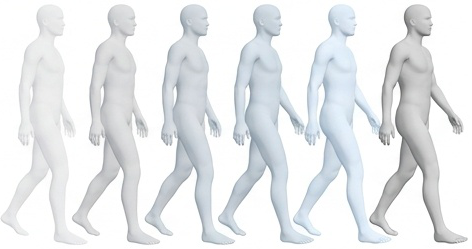
\includegraphics[width=28mm]{figures/architecture_motion.png}};
\draw[line] (dec.south) -- (motOut.north);
\node[lbl,below=1pt of motOut] {generated motion $\hat{\mathbf{x}}$};

% =====================================================================
% legend
% =====================================================================
\begin{scope}[shift={(0,-8.9)},font=\sffamily\scriptsize,
    sw/.style={minimum width=3.5mm,minimum height=2mm,inner sep=0pt,rounded corners=1.5pt,line width=0.5pt},
    tk/.style={minimum size=1.6mm,inner sep=0pt,draw=ink,line width=0.35pt},
    lt/.style={anchor=west,inner sep=1.5pt,text=ink}]
  \node[sw,fill=egofill,draw=egoedge] (l1) at (0.2,0) {};
  \node[lt] (t1) at (l1.east) {pretrained in (a), frozen in (b)};
  \node[sw,fill=denfill,draw=denedge,right=5mm of t1] (l2) {};
  \node[lt] (t2) at (l2.east) {trained in (b)};
  \node[sw,fill=vaefill,draw=vaeedge,dashed,right=5mm of t2] (l3) {};
  \node[lt] (t3) at (l3.east) {pretrained motion VAE, frozen throughout};
  \node[tk,fill=lattok,right=7mm of t3] (l4) {};
  \node[lt] (t4) at (l4.east) {motion latent};
  \node[tk,fill=timetok,right=4mm of t4] (l5) {};
  \node[lt] (t5) at (l5.east) {timestep};
  \node[tk,fill=egotok,right=4mm of t5] (l6) {};
  \node[lt] (t6) at (l6.east) {ego token};
  \node[tk,fill=motfill,right=4mm of t6] (l7) {};
  \node[lt] (t7) at (l7.east) {body motion};
\end{scope}
\end{tikzpicture}
}
  \caption{\method architecture. \textbf{(a) Ego-encoder pretraining.} The ego encoder (1) is trained so that its mean-pooled, projected output $\bar{\mathbf{c}}$ matches the mean-pooled posterior mean $\bar{\mathbf{z}}$ of the frozen motion VAE for the paired motion. \textbf{(b) Latent diffusion.} The ego encoder is \emph{frozen} and produces the single pooled token $\bar{\mathbf{c}}$. At every denoising step the $L=4$ noisy latent tokens $\mathbf{z}_t$, the timestep embedding and $\bar{\mathbf{c}}$ form one 6-token sequence for a self-attention transformer denoiser (2), whose first four output tokens predict the noise. The \fullseq ablation skips the pooling and passes all 196 encoder tokens.}
  \label{fig:architecture}
\end{figure*}

\subsection{Problem Formulation}

Given an ego-vehicle trajectory $\mathbf{e} \in \mathbb{R}^{T \times 2}$, the vehicle's ground-plane position over $T=196$ frames at 20\,fps expressed in the pedestrian's initial frame, we generate pedestrian body motion $\mathbf{x} \in \mathbb{R}^{T \times 263}$ in the HumanML3D representation~\cite{guo2022humanml3d}, which encodes root velocity and rotation, joint positions and velocities and foot contacts.
We model $p(\mathbf{x} \mid \mathbf{e})$ with a latent diffusion model (Fig.~\ref{fig:architecture}).

\subsection{Motion VAE}

We use the MLD VAE~\cite{chen2023mld}, a transformer encoder--decoder that compresses $T \times 263$ motion into $L = 4$ latent tokens of 256 dimensions.
We train it from scratch on the training partition of our data (Section~\ref{sec:data}) for 6{,}000 epochs, with features normalised by that partition's statistics, and keep it frozen afterwards.

\subsection{Ego Encoder}
\label{sec:egoencoder}

A lightweight transformer encodes the ego trajectory. A linear projection from 2 to 256 dimensions, sinusoidal positional encoding and four encoder layers with four heads give $\mathbf{c} \in \mathbb{R}^{196 \times 256}$.
\method mean-pools $\mathbf{c}$ over time and applies a two-layer projection head, giving one conditioning token $\bar{\mathbf{c}} \in \mathbb{R}^{256}$, analogous to a pooled text embedding.

\paragraph{Pretraining.}
Before diffusion training, the encoder is trained to regress the paired motion's latent. With $\bar{\mathbf{z}}$ the mean-pooled VAE posterior mean, the loss is
\begin{equation}
  \mathcal{L}_{\mathrm{pre}} = \|\bar{\mathbf{c}} - \bar{\mathbf{z}}\|^2 + \lambda\bigl(1 - \cos(\bar{\mathbf{c}}, \bar{\mathbf{z}})\bigr), \quad \lambda = 0.1 .
\end{equation}
The encoder is then \emph{frozen} during diffusion training.
Section~\ref{sec:design} tests both choices, together with a \fullseq variant that skips the pooling and lets the denoiser attend to all 196 tokens.

\subsection{Denoiser and Guidance}

The MLD denoiser is a self-attention transformer (9 layers, 4 heads, 256 dimensions) over the concatenation of the noisy latent tokens, the timestep embedding and the condition. The first $L$ output tokens predict the noise,
\begin{equation}
  \hat{\boldsymbol{\epsilon}} = \mathrm{Transformer}\bigl([\mathbf{z}_t,\, \mathbf{t}_{\mathrm{emb}},\, \bar{\mathbf{c}}]\bigr)_{1:L}.
\end{equation}
It is trained with the DDPM noise-prediction loss $\mathbb{E}\,\|\boldsymbol{\epsilon} - \hat{\boldsymbol{\epsilon}}\|^2$ (1{,}000 steps) and sampled with 50 DDIM steps~\cite{song2021ddim}.
For classifier-free guidance~\cite{ho2022cfg}, the ego input is zeroed for 10\% of training samples, so the encoder's response to the all-zero trajectory is the unconditional embedding, and at inference
\begin{equation}
  \hat{\boldsymbol{\epsilon}}_w = \boldsymbol{\epsilon}_\theta(\mathbf{z}_t, \emptyset) + w \bigl(\boldsymbol{\epsilon}_\theta(\mathbf{z}_t, \bar{\mathbf{c}}) - \boldsymbol{\epsilon}_\theta(\mathbf{z}_t, \emptyset)\bigr).
\end{equation}

%----------------------------------------------------------------------
\section{DATA}
\label{sec:data}
%----------------------------------------------------------------------

\subsection{Sources and Processing}

No dataset pairs vehicle trajectories with pedestrian body motion, so we built one from two complementary sources. The public driving datasets nuScenes~\cite{caesar2020nuscenes} and Waymo~\cite{sun2020waymo} supply scale and behavioural diversity, and a small set of deliberately \emph{staged} high-interaction scenes recorded with our research vehicle (LiDAR, surround cameras and GNSS) targets close-range encounters that are rare in public data.
We staged 17 scenarios on public roads, such as crossing in front of the vehicle, stopping at the kerb or hesitating while it approaches, brakes or turns. The pedestrian in these scenes is one of the authors, who consented to the recording and its release.
The recordings are converted to the nuScenes format and annotated with 3D boxes and orientations using MS3D~\cite{tsai2024ms3d++,tsai2023ms3d}.

For every annotated pedestrian in all three sources we estimate SMPL~\cite{SMPL:2015} poses with an adapted OmniRe~\cite{chen2025omnire}, localising the person in every camera through the projected 3D box and stitching the per-camera estimates into one sequence with the rig calibration. The root position comes from this fit.
The poses are converted to the 263-dimensional HumanML3D representation~\cite{guo2022humanml3d}, which retargets every sequence onto one canonical skeleton, so body shape is not represented.
One pipeline resamples body motion and ego odometry to 20\,fps and expresses both in a pedestrian-centric frame, translated and yaw-normalised to the pedestrian's first pose.
Every sequence is also stored mirrored left to right.
Sequences longer than 196 frames are windowed (about 40\%), shorter ones are padded and masked. A window keeps the frame of its track's first pose, which on test lies a median 1.7\,m from the pedestrian's position at the window start (43\% of conditions). Tracks shorter than 2\,s are replaced by their neighbour in the list, so the 1{,}182 test rows we score hold 1{,}146 distinct conditions. Dropping the 36 repeats changes no per-condition number by more than 0.02.

\subsection{Scene-Level Split}

All partitions are split by scene, so a scene, every pedestrian in it and every mirrored copy stay on one side (Table~\ref{tab:dataset}).
In a file-level split of the same data, the mirrored twin of 83\% of the held-out sequences was in the training set.
We selected models on the validation partition and evaluated the test partition once, after all selection was fixed.
The staged scenes contribute only six sequences to each held-out partition, so held-out results speak for nuScenes and Waymo.

\begin{table}[t]
  \centering
  \caption{Dataset composition, counted with mirrored copies (5{,}668 recorded sequences, each mirrored once). Each sequence pairs an ego trajectory ($196\times2$) with pedestrian body motion ($196\times263$). Partitions share no scene.}
  \label{tab:dataset}
  \vspace{4pt}
  \small
  \setlength{\tabcolsep}{6pt}
  \begin{tabular}{lcccc}
    \toprule
    Source & Train & Validation & Test & Total \\
    \midrule
    Staged (ours) & 20 & 6 & 6 & 32 \\
    nuScenes & 3{,}512 & 462 & 446 & 4{,}420 \\
    Waymo Open Dataset & 5{,}506 & 684 & 694 & 6{,}884 \\
    \midrule
    Sequences & 9{,}038 & 1{,}152 & 1{,}146 & 11{,}336 \\
    Scenes & 796 & 107 & 91 & 994 \\
    \bottomrule
  \end{tabular}
\end{table}

\paragraph{Interaction-aware data recipe (IA).}
As a data-side alternative we test a recipe that concentrates training on interactions. Each sequence gets an interaction score $s = s_{\text{travel}}\, s_{\text{prox}}\, s_{\text{bearing}}$ from the pedestrian's path length, the fraction of frames within 5\,m of the vehicle and the swept relative bearing ($1 + \sum_t|\Delta\phi_t|/180^\circ$). IA samples training sequences with probability proportional to $s$ (floored at 0.01) and centres the 196-frame window on the closest approach, with $\pm25\%$ jitter. Without IA, sequences are drawn uniformly and windows at random. Evaluation always uses one fixed window per sequence, identical for every model.

\subsection{Pose-Label Audit}
\label{sec:posequality}

The pose labels are estimates, and no reference such as mocap exists for these scenes. We therefore audit what can be checked without one, on all 13{,}958 scorable sequences we extracted, a superset of those in Table~\ref{tab:dataset}.
First, \textbf{body shape was never estimated}. Every sequence shares one skeleton to within $10^{-5}$ relative bone length.
Second, \textbf{the feet do not plant}. During locomotion one foot should be stationary, yet the slowest foot joint moves at a median $0.97$ of root speed ($0$ = clean footfalls, $1$ = the body sliding as a rigid unit), and $94.6\%$ of moving sequences never hold a foot still for more than $5\%$ of their frames.
Third, \textbf{articulation is damped}. Against HumanML3D's mocap statistics, root translation varies more ($1.29\times$) but root-relative joint positions, root height and turning far less ($0.44\times$, $0.26\times$, $0.37\times$). Part of that gap is content, since our data is people walking near roads.
A pilot that re-solves the legs against the root removes the sliding (skate 0.15), so relabelling is viable and left to future work.

The consequence for evaluation is direct. The body is a lightly articulated canonical template sliding along the root path, so our conditioning evidence, trajectory error and stopping decisions, is computed from the root. The root itself has no independent reference. The labels hold no head yaw, and head turns in the raw body fits look like a bias of the vehicle-mounted cameras rather than attention, so we make no claim about orientation. FID scores the body against this damped target and should be read as a within-benchmark comparison only.

%----------------------------------------------------------------------
\section{EVALUATION PROTOCOL}
\label{sec:eval}
%----------------------------------------------------------------------

\paragraph{Distributional metrics.}
FID, Diversity and MultiModality (MM) follow the HumanML3D protocol~\cite{guo2022humanml3d}, with its pretrained motion encoders as feature extractor. Diversity is the mean pairwise distance across generated samples (closer to the ground truth's 5.26--5.40 is better), and MM the mean pairwise distance among 10 samples of one condition. Each is the mean of three generation passes. We do not report R-Precision. It retrieves with each model's own ego encoder, so it is not comparable across encoders, and it falls to chance for a trainable encoder.

\paragraph{Per-condition metrics.}
For each test condition we draw $K{=}5$ samples, take the pelvis ground-plane path and compare it with the recorded pedestrian over the true sequence length. The average and final displacement errors (ADE, FDE) are means over the samples, and minADE and minFDE take the best of five. Mean ADE rewards samples that concentrate on the likely outcome, min-of-$K$ rewards coverage, so we read them together.

\paragraph{Ego-Coupling Score.}
\label{sec:behavior}
A pedestrian \emph{stops} if the root speed stays below 0.2\,m/s for at least 1\,s. For condition $\mathbf{e}$, $\hat{p}(\mathrm{stop}\mid\mathbf{e})$ is the fraction of the $K$ samples that stop. The Ego-Coupling Score (ECS) is the mean of $\hat{p}$ over conditions whose recorded pedestrian stops minus its mean over conditions whose pedestrian walks. It is 0 for a model that ignores the vehicle and 1 for perfect coupling. A predictor that stops too often can also score high, so we always report the Brier score of $\hat{p}$ against the recorded label with it. From that score we subtract the sampling noise of the $K$ draws, $\hat{p}(1-\hat{p})/(K-1)$ per condition, which otherwise penalises a model for spreading its samples. We adopted this correction after the test pass (uncorrected, \method scores 0.191 and the prior 0.214). Stopping occurs in 24\% of test conditions, whereas crossing the vehicle's path occurs in only about 2\% and is too rare to score.

\paragraph{Seeds, statistics and selection.}
The four main models and the two encoder ablations are trained with three seeds each, the two priors and the trainable \fullseq run with one. Each seed's checkpoint is the one with the lowest validation FID among 50 saved every 100 epochs, and each model's guidance scale is the one in $\{5, 10, 15\}$ with the lowest validation FID averaged over its seeds. Unconditional models see the real ego trajectory during training-time validation, so their checkpoints are chosen by an offline validation pass with the ego zeroed.
Contrasts average a model's seeds and resample scenes (2{,}000 scene-clustered bootstrap draws), because pedestrians of one scene are not independent. Before the test partition was used, we fixed one rule. A model beats another only if the 95\% interval excludes zero \emph{and} all seed pairs agree in sign, nine between two three-seed models and three against a single-seed model. The bootstrap captures sampling of scenes but not of seeds, which the second condition covers. The primary contrast is \method against \fullseq on mean ADE.

%----------------------------------------------------------------------
\section{RESULTS}
\label{sec:results}
%----------------------------------------------------------------------

\begin{table*}[t]
  \centering
  \caption{Test partition (1{,}182 scored rows, 91 scenes), mean over three seeds with the seed range in brackets. FID, Diversity and MultiModality (MM) use the HumanML3D evaluator, and ADE to Brier are per-condition metrics from $K{=}5$ samples. Ground-truth Diversity is 5.26--5.40. Bold marks the best of the four main models in each column except Diversity and MM.}
  \label{tab:main}
  \vspace{4pt}
  \small
  \setlength{\tabcolsep}{2.4pt}
  \begin{tabular}{lccc|cccccc}
    \toprule
    Model & FID $\downarrow$ & Div. & MM & ADE $\downarrow$ & FDE $\downarrow$ & minADE $\downarrow$ & minFDE $\downarrow$ & ECS $\uparrow$ & Brier $\downarrow$ \\
    \midrule
    \method & 5.67\ci{5.36}{6.26} & 5.63 & 3.10 & \textbf{2.43}\ci{2.38}{2.48} & \textbf{5.11} & 1.65\ci{1.59}{1.74} & 3.40 & \textbf{0.31}\ci{0.29}{0.34} & 0.180 \\
    \fullseq & 4.16\ci{2.96}{4.91} & 5.78 & 3.92 & 2.69\ci{2.52}{2.98} & 5.67 & \textbf{1.54}\ci{1.49}{1.57} & \textbf{3.18} & 0.27\ci{0.24}{0.29} & \textbf{0.162} \\
    \method + IA & 4.84\ci{4.69}{5.04} & 5.83 & 3.22 & 2.93\ci{2.86}{3.03} & 6.23 & 2.04\ci{1.98}{2.13} & 4.29 & 0.21\ci{0.18}{0.25} & 0.186 \\
    \fullseq + IA & \textbf{3.24}\ci{2.73}{4.14} & 5.89 & 3.21 & 3.01\ci{2.82}{3.14} & 6.50 & 2.07\ci{1.72}{2.31} & 4.42 & 0.10\ci{0.06}{0.12} & 0.202 \\
    \fullseq, encoder trainable (1 seed) & 6.54 & 5.32 & 4.66 & 2.67 & 5.55 & 1.39 & 2.79 & 0.04 & 0.195 \\
    \midrule
    Trained prior (no ego, 1 seed) & 4.67 & 5.79 & 5.23 & 3.11 & 6.38 & 1.31 & 2.64 & 0.02 & 0.179 \\
    Trained prior + IA (1 seed) & 3.29 & 5.47 & 4.76 & 3.00 & 6.30 & 1.52 & 3.09 & 0.01 & 0.205 \\
    \bottomrule
  \end{tabular}
\end{table*}

\begin{table*}[t]
  \centering
  \caption{Contrasts on the test partition as the difference of seed means, positive when the first model is better, with 95\% scene-bootstrap interval. $^\ast$ meets the rule fixed before the test pass (interval excludes 0, all seed pairs agree in sign).}
  \label{tab:contrasts}
  \vspace{4pt}
  \small
  \setlength{\tabcolsep}{8pt}
  \begin{tabular}{lccc}
    \toprule
    Contrast & ADE (m) & minADE (m) & ECS \\
    \midrule
    \method vs.\ \fullseq & $+0.26^\ast$\ci{0.17}{0.33} & $-0.11^\ast$\ci{-0.18}{-0.05} & $+0.04$\ci{0.00}{0.08} \\
    \method+IA vs.\ \fullseq+IA & $+0.08$\ci{-0.04}{0.20} & $+0.03$\ci{-0.08}{0.15} & $+0.11^\ast$\ci{0.05}{0.18} \\
    \method vs.\ \method+IA & $+0.50^\ast$\ci{0.30}{0.70} & $+0.39^\ast$\ci{0.20}{0.57} & $+0.09^\ast$\ci{0.02}{0.16} \\
    \fullseq vs.\ \fullseq+IA & $+0.31$\ci{0.11}{0.55} & $+0.53^\ast$\ci{0.34}{0.74} & $+0.17^\ast$\ci{0.09}{0.25} \\
    \method vs.\ prior & $+0.68^\ast$\ci{0.49}{0.86} & $-0.34^\ast$\ci{-0.46}{-0.22} & $+0.29^\ast$\ci{0.19}{0.39} \\
    \fullseq vs.\ prior & $+0.42^\ast$\ci{0.22}{0.63} & $-0.23^\ast$\ci{-0.34}{-0.12} & $+0.26^\ast$\ci{0.16}{0.34} \\
    \method+IA vs.\ prior+IA & $+0.07$\ci{-0.23}{0.34} & $-0.52^\ast$\ci{-0.77}{-0.28} & $+0.21^\ast$\ci{0.13}{0.30} \\
    \fullseq+IA vs.\ prior+IA & $-0.01$\ci{-0.29}{0.25} & $-0.55^\ast$\ci{-0.80}{-0.33} & $+0.09^\ast$\ci{0.04}{0.15} \\
    \bottomrule
  \end{tabular}
\end{table*}

\subsection{\method Uses the Vehicle}
\label{sec:main}

Table~\ref{tab:main} gives the test results and Table~\ref{tab:contrasts} the contrasts.
Against a prior trained on the same data without the ego trajectory, \method lowers mean ADE by 0.68\,m (3.11 to 2.43\,m) and FDE by 1.27\,m, and raises the Ego-Coupling Score from 0.02 to 0.31, with every seed pair agreeing.
The prior is better on minADE, as any sampler that spreads its five samples widely must be, so minADE alone is no test of conditioning.
The coupling is the same on validation (ECS 0.36 against 0.02) and holds on both large sources (test ECS 0.32 on nuScenes and 0.26 on Waymo, against $-$0.01 and 0.04 for the prior). It is specific to the vehicle in the scene. Given another scene's vehicle, \method falls to the prior's level (Section~\ref{sec:controls}).

\subsection{FID Does Not See the Conditioning}
\label{sec:fid}

Read by FID, Table~\ref{tab:main} tells a different story. The best FID belongs to \fullseq+IA (3.24), with the ego-blind prior trained on the same recipe level with it (3.29), and \method has the worst FID of the four conditional cells (5.67) while being the most accurate on mean ADE and at least as strongly coupled. Across the nine models of Tables~\ref{tab:main} and~\ref{tab:design}, with seeds averaged, the rank correlation of FID with mean ADE is $-0.75$ ($p = 0.02$), so the lower a model's FID, the larger its trajectory error. Fig.~\ref{fig:fidade} shows the single runs of Table~\ref{tab:main}, which are not independent. FID and ECS are not significantly related ($+0.33$, $p = 0.38$). Interaction-weighted data illustrates the mechanism. It lowers FID for the conditional model and the prior alike, because it changes which motions the model sees, and at the same time it worsens mean ADE, minADE and ECS for both encoders (Table~\ref{tab:contrasts}, rows 3--4, five of six under our rule), and the IA models are no better than their own prior on mean ADE. A metric of the marginal can reward a change that removes conditioning. We therefore select checkpoints by FID, as is standard, but rank models only by the per-condition metrics.

\begin{figure}[t]
  \centering
  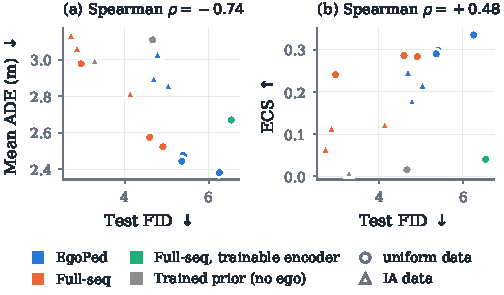
\includegraphics[width=\linewidth]{figures/fid_vs_conditioning.pdf}
  \caption{Test FID against per-condition accuracy, one point per training run (15 runs, colour for model, marker for data recipe). Lower FID goes with \emph{larger} trajectory error (a), its relation to coupling (b) is weaker, and the ego-blind prior on IA data sits among the best FIDs.}
  \label{fig:fidade}
\end{figure}

\subsection{Encoder Design}
\label{sec:design}

\paragraph{Pooled against full-sequence conditioning.}
Letting the denoiser attend to all 196 encoder tokens instead of one pooled token makes per-condition predictions worse on average. \fullseq trails \method by 0.26\,m in mean ADE (Table~\ref{tab:contrasts}), the pre-specified primary contrast, and did so on validation as well (0.37\,m). The trade-off is spread. \fullseq's samples cover more outcomes (MM 3.92 vs.\ 3.10, better minADE by 0.11\,m), its FID is lower and its Brier score is better on test (0.162 vs.\ 0.180, level on validation), at 201 instead of 6 tokens per denoising step. On coupling the two encoders are close without IA (ECS 0.27 vs.\ 0.31, below our rule on test, met on validation), and \method couples clearly better with IA (0.21 vs.\ 0.10). A likely cause is pretraining, which aligns only the pooled token and never the 196 per-frame tokens.

\paragraph{Freezing and pretraining.}
Table~\ref{tab:design} reports \method with its encoder trained together with the denoiser, initialised from pretraining or from scratch, three seeds each, selected like every other model.
Freezing matters. The frozen encoder beats the trainable pretrained one on all four per-condition metrics under our rule (before rounding, ADE by 0.09\,m, minADE by 0.25\,m and ECS by 0.07), and on validation on all but ADE, while FID does not separate the two (5.67 vs.\ 5.65).
Pretraining by itself does not help. Once the encoder is trainable, pretrained and scratch initialisation give the same result on every metric and on both partitions, so the pretrained representation helps only as long as diffusion training cannot change it.
The trainable encoders also concentrate their samples (MM 2.03 and 2.15 against 3.10), which costs minADE without improving the mean.
Validation FID selected early checkpoints for four of the six trainable runs (epochs 999--1099), so we decided before the test pass to also report the last checkpoint. It shows the same picture with worse FID, and the ADE gap to the frozen encoder (0.07\,m) no longer meets the rule.
A single-seed \fullseq run with a trainable encoder, by contrast, stays close to ego-blind (ECS 0.04 against 0.27 frozen, Table~\ref{tab:main}).

\begin{table}[t]
  \centering
  \caption{Encoder ablations of \method on the test partition, means over three seeds. Upper rows use the checkpoint and guidance selected on validation like every other model (guidance 15, 15, 10). Lower rows use the last checkpoint of the same runs at the same guidance, reported as decided before the test pass.}
  \label{tab:design}
  \vspace{4pt}
  \footnotesize
  \setlength{\tabcolsep}{3pt}
  \begin{tabular}{lccccc}
    \toprule
    Encoder & FID $\downarrow$ & MM & ADE $\downarrow$ & minADE $\downarrow$ & ECS $\uparrow$ \\
    \midrule
    Pretrained, frozen (\method) & 5.67 & 3.10 & 2.43 & 1.65 & 0.31 \\
    Pretrained, trainable & 5.65 & 2.15 & 2.53 & 1.90 & 0.23 \\
    From scratch, trainable & 5.77 & 2.03 & 2.50 & 1.87 & 0.24 \\
    \midrule
    \multicolumn{6}{l}{\textit{Last checkpoint (epoch 4{,}999)}} \\
    Pretrained, trainable & 6.78 & 1.64 & 2.51 & 2.01 & 0.23 \\
    From scratch, trainable & 7.03 & 1.74 & 2.50 & 1.97 & 0.23 \\
    \bottomrule
  \end{tabular}
\end{table}

\subsection{Which Part of the Trajectory Is Used}
\label{sec:controls}

Table~\ref{tab:controls} gives \method's three seeds manipulated ego input, without retraining.
Given the trajectory of a vehicle from another scene, \method is no better than the trained prior (ADE 3.09 against 3.11\,m) and its coupling vanishes (ECS 0.00). Its Brier score (0.30) is far worse than the prior's (0.18), because it reacts confidently to the wrong vehicle. Zeroing the input gives the prior's numbers too. A vehicle that stays at its start position removes most of the coupling as well (ECS 0.06), so the model reacts to how the vehicle moves, not only to where it is.
Showing only the first second and continuing it at constant velocity keeps the coupling (ECS 0.31 on test, 0.30 against 0.36 on validation, not a difference under our rule) and most of the gain in ADE (2.60\,m, between 2.43 with the full trajectory and 3.04 with a stationary vehicle). The stop decision is thus carried by the vehicle's early motion, and its later trajectory refines the path. The ADE cost of the 1\,s horizon meets our rule on both partitions, as do all differences between the full input and the stationary, foreign or zeroed vehicle.

\begin{table}[t]
  \centering
  \caption{Ego controls for \method on the test partition (three seeds at their selected checkpoints, no retraining). Horizon rows show the first $S$ seconds of the ego trajectory and continue it at the velocity of the last 0.5\,s. The prior row is the separately trained model for reference.}
  \label{tab:controls}
  \vspace{3pt}
  \footnotesize
  \setlength{\tabcolsep}{3pt}
  \begin{tabular}{lcccc}
    \toprule
    Ego input & ADE $\downarrow$ & minADE $\downarrow$ & ECS $\uparrow$ & Brier $\downarrow$ \\
    \midrule
    Full trajectory (9.8\,s) & 2.43 & 1.65 & 0.31 & 0.180 \\
    First 2\,s, then constant velocity & 2.52 & 1.74 & 0.33 & 0.184 \\
    First 1\,s, then constant velocity & 2.60 & 1.81 & 0.31 & 0.195 \\
    Vehicle stationary at its start & 3.04 & 2.07 & 0.06 & 0.231 \\
    Vehicle from another scene & 3.09 & 2.31 & 0.00 & 0.302 \\
    Zeroed (unconditional branch) & 3.03 & 1.31 & 0.03 & 0.177 \\
    \midrule
    Trained prior (no ego) & 3.11 & 1.31 & 0.02 & 0.179 \\
    \bottomrule
  \end{tabular}
\end{table}

\subsection{What the Coupling Rests On}
\label{sec:rests}

We probed the score with definitions fixed on validation. First, 57\% of the recorded stops are pedestrians who stand throughout, within a 1\,m radius. \method gives them a stop probability of 0.55, against 0.30 for those who move and then stop and 0.13 for walkers, and its lead over the prior in the middle group (ECS 0.17 against 0.05) meets our rule on validation but not on test.
Second, in 99\% of the test conditions the pedestrian never comes within 2.5\,m of where the vehicle is or later drives (median closest approach 10.4\,m), and there \method keeps its ECS (0.31 against 0.02) and its ADE gain (0.68\,m). The recording vehicle thus cannot have revealed the outcome by reacting to the pedestrian, but for the same reason the data holds almost no interaction.
Third, part of the signal is geometry. Walkers mostly face along the road, so 9\% of pedestrians stop when the vehicle travels within $10^\circ$ of the axis they face and 40\% beyond $60^\circ$. Within bins of this angle \method keeps an ECS of 0.17 (0.29 on validation). A rule that predicts a stop unless the vehicle travels within $10^\circ$ of that axis even reaches an ECS of 0.29, but it predicts a stop for 65\% of the conditions and has a Brier score of 0.47.
Finally, the Brier score does not separate \method (0.180) from the prior (0.179) on test, although it does on validation (0.156 against 0.171), while \method ranks conditions better on both (area under the ROC curve 0.70 against 0.52 on test).
The coupling is thus a statistical dependence on the vehicle's motion and the geometry it reveals, strongest for pedestrians who stand, and not a measured reaction to the vehicle.

\subsection{Guidance}

Guidance trades coverage for FID without changing coupling. On validation, raising $w$ from 5 to 15 lowers \method's FID from 4.61 to 3.90 but raises its minADE from 1.22 to 1.43\,m and its ADE by 0.03\,m, while ECS stays flat (0.36--0.37). \fullseq behaves alike. Selecting the scale by FID, as our protocol does, therefore picks the least accurate setting. We keep the pre-specified selection.

\begin{figure*}[t]
  \centering
  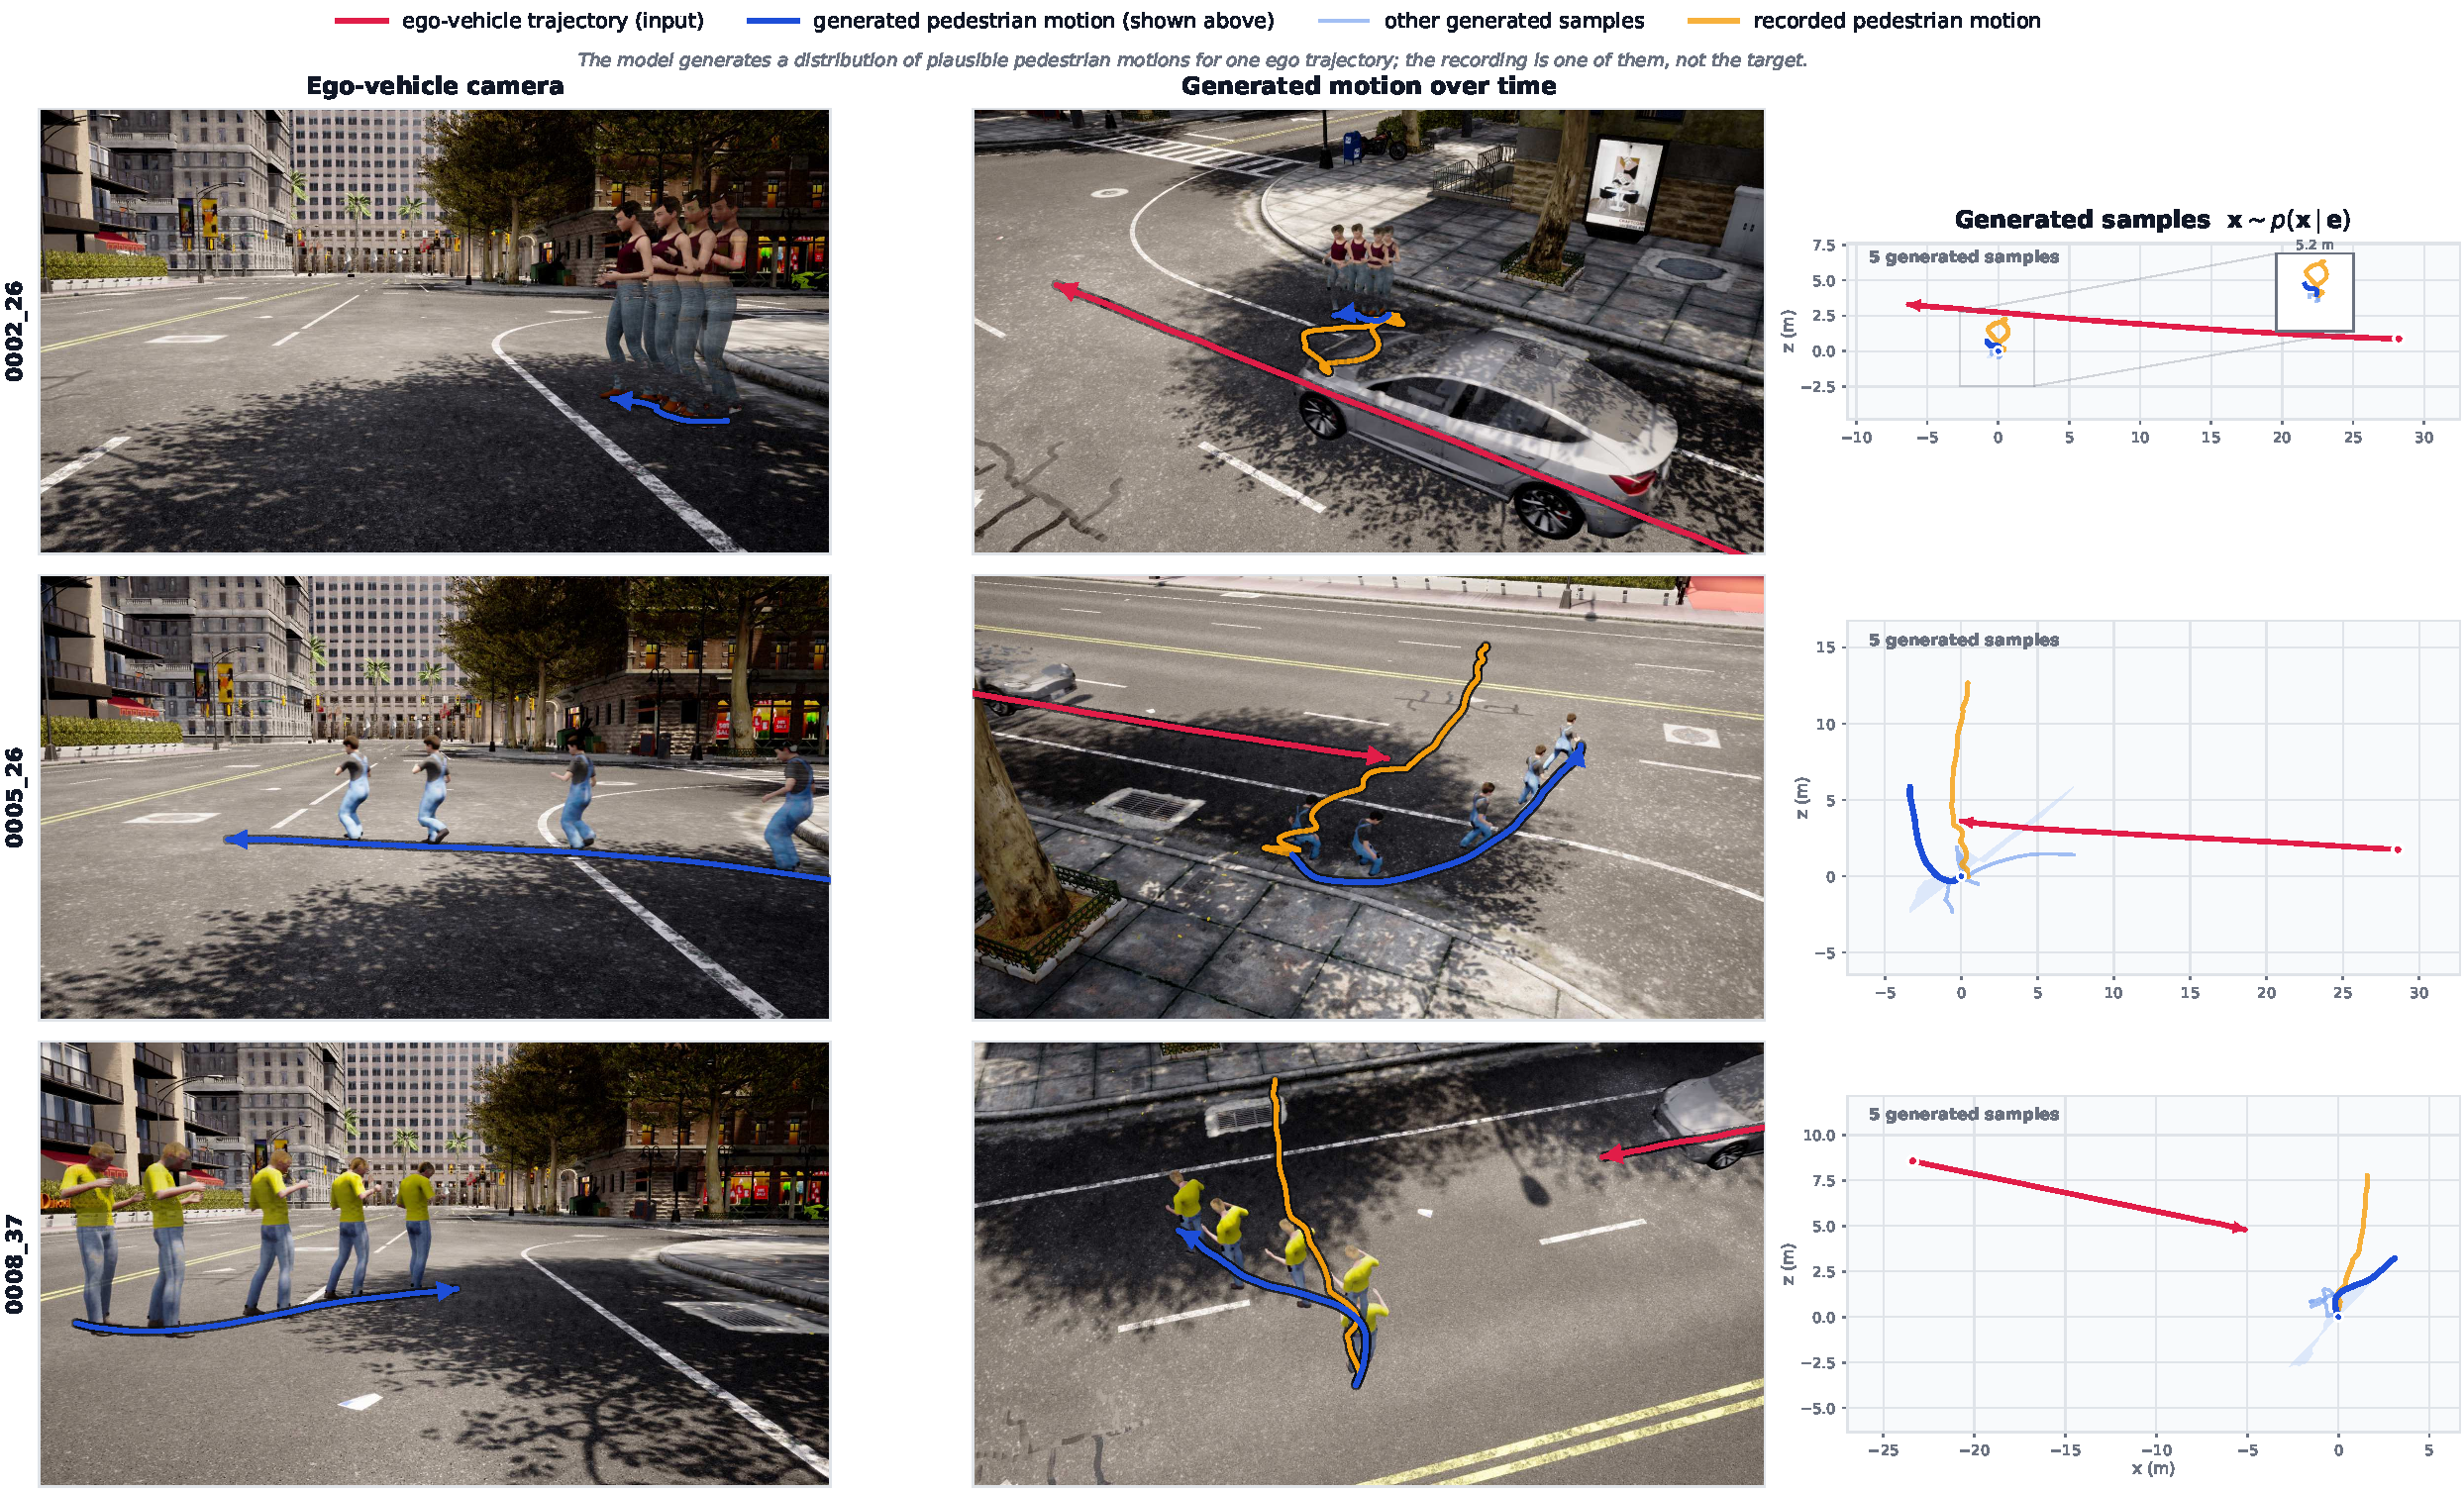
\includegraphics[width=\linewidth]{figures/FINAL_setA_compressed.pdf}
  \caption{\TODO{Placeholder from an earlier model, to be replaced (test conditions, anonymous, no taller than this).} Generated body motion retargeted onto pedestrian characters in the CARLA simulator~\cite{dosovitskiy2017carla}, one ego condition per row. The left column shows the view from the ego vehicle, the middle column a third-person view over time with the ego trajectory (red), the shown sample's root path (dark blue) and the recorded pedestrian (orange), and the right column a bird's-eye view of five samples for the same ego trajectory. The recording is one outcome of the distribution, not its target, and the feet slide as in the labels (Section~\ref{sec:posequality}).}
  \label{fig:qualitatives}
\end{figure*}

\subsection{Comparison with PedGen}
\label{sec:pedgen}

The released context-free model of PedGen~\cite{liu2025pedgen} cannot take a vehicle trajectory, so we use it as an ego-blind reference on the root path, the one quantity both models share. We compare paths over the first 1.95\,s of our test conditions, within PedGen's 2-second horizon. With $K{=}5$ samples, mean ADE is 0.575\,m for \method, 0.632\,m for \fullseq, 0.750\,m for our trained prior and 0.794\,m for PedGen's context-free model. \method is 0.22\,m closer than PedGen, with the interval excluding zero for every seed. Even our ego-blind prior is level with PedGen, so part of the gap is the domain. PedGen's samples walk at a median 0.65\,m/s against 1.26\,m/s in our data. The comparison shows that a published generator does not transfer to this setting without retraining, not that one architecture is better than the other.

\subsection{Qualitative Results}

Fig.~\ref{fig:teaser} shows one \method model under two vehicle trajectories with the same noise, and Fig.~\ref{fig:qualitatives} shows generated motion in a simulator.
\TODO{For visualisation, the generated HumanML3D joint sequences are retargeted onto CARLA pedestrian skeletons and replayed in a CARLA town together with an ego vehicle that follows the conditioning trajectory [Mohan, please describe the retargeting and scene placement, CARLA version and town briefly].}

%----------------------------------------------------------------------
\section{DISCUSSION AND LIMITATIONS}
\label{sec:discussion}
\label{sec:limitations}
%----------------------------------------------------------------------

Had we ranked by FID, this paper would recommend full-sequence attention with interaction-weighted data, the combination with the weakest coupling to the vehicle among our four main models. A split that shares no scene, a rule over several seeds and per-condition metrics that an ego-blind model cannot pass prevent that conclusion. For conditional motion generation in general, we suggest reporting a separately trained unconditional prior on the same data recipe and at least one per-condition metric next to FID.

\begin{itemize}
  \item \textbf{Body pose quality.} The labels have one canonical skeleton, feet that do not plant and damped articulation (Section~\ref{sec:posequality}). Relabelling and retraining is the largest open item.
  \item \textbf{Observational coupling.} The coupling is measured on recordings in which almost no pedestrian is in the vehicle's path (Section~\ref{sec:rests}). How the model responds to a plan that was never driven is untested, and for windowed tracks the vehicle is given in the frame of the track's first pose.
  \item \textbf{Known future.} \method sees the vehicle's whole 9.8\,s trajectory, which suits simulation but not online prediction.
  \item \textbf{Condition and coverage.} The condition is the ego trajectory only, without map, other agents or traffic control, and held-out results rest on nuScenes and Waymo. The input is the 2D trajectory of any moving agent, so mobile robots are a natural next use after retraining on data such as JRDB~\cite{martinmartin2023jrdb}.
  \item \textbf{Metrics.} ECS covers only stopping, because crossing is too rare in our windows to score. FID values compare only within this benchmark, and we report no perceptual study.
\end{itemize}

%----------------------------------------------------------------------
\section{CONCLUSION}
%----------------------------------------------------------------------

\method generates full-body pedestrian motion from the ego vehicle's trajectory with a pretrained, frozen, pooled trajectory encoder and latent diffusion. Against a prior trained without the vehicle, it lowers trajectory error by 0.68\,m and lifts the coupling of generated stopping decisions from 0.02 to 0.31. This coupling is observational and rests mostly on pedestrians who stand, so reactions to an unrecorded vehicle plan remain to be tested. The same experiments show that FID cannot certify such a model. It favours the design choices that raise mean trajectory error and places an ego-blind prior level with the best conditional model. Per-condition trajectory error and the Ego-Coupling Score, with scene-level statistics over several seeds, are what we propose for evaluating generation conditioned on another agent. Code, trained models and data will be released.

%----------------------------------------------------------------------
\ifanonymous\else
\section*{ACKNOWLEDGMENT}
This work is a result of the joint research project STADT:up (grant no.\ 19A22006N). The project is supported by the German Federal Ministry for Economic Affairs and Climate Action (BMWK), based on a decision of the German Bundestag. The authors are solely responsible for the content of this publication.
\fi

\bibliographystyle{IEEEtran}
\bibliography{ral_ctl,refs}

\end{document}
